\documentclass[../main.tex]{subfiles}
\graphicspath{{\subfix{../../images/}}}

\begin{document}

The internet is one of the most influential creations of society. It has impacted all of us in some way. This section will focus on it. The internet at its core is just a bunch of computers connected together over a very large wide-area network (WAN), hence the words INTERconnected NETwork.

\subsection{The Internet vs the Worldwide Web (WWW)}

Internets come from the words Interconnected Network; they are literally just computers connected together that can share data amongst themselves. If I took 5 laptops and connected each of them to each other, that would technically be an internet. The internet has some protocols (rules) that are defined for computers to communicate in a uniform way.

\begin{itemize}
    \item The internet that we know of is the largest collection of computers that are connected together. They consist of servers, which provide the websites and services, and they are all connected to each other in some way.
    \item The internet is more of a concept that a tangible thing; the servers that you can touch are just computers. The connection between the servers is what the internet really is. However, \textbf{it still relies on a tangible infrastructure.}
\end{itemize}

The World Wide Web (or WWW) is just a part of the internet that we can access. The world wide web consist of the things that sit on top of the internet, all the web pages and services like Google, YouTube, Discord, Reddit, Instagram, etc. are a part of the WWW. The WWW also provides extra protocols on top of the internet's protocols that relate to the content on the WWW, like how websites should be written, encryption, etc.

In summary, the internet are the connections between physical infrastructure that provide the technology for computers to communicate, and the WWW are the webppages, content and protocols that sits on top of the internet's protocols.

\subsection{URLs (Uniform Resource Locators)}

Web browsers, or just browsers allows you to view content on the WWW. Browsers interpret HTML\footnote{Hypertext Markup Langauge}, which is a specific programming language that defines the basic component and the text in a webpage, think the bricks in your house. To access these files, the browser must visit a URL, which locates a location on the WWW. They look as follows:

\begin{figure}[H]
    \centering
    
\includegraphics[width=0.7\textwidth]{url.png}
    \caption{The parts of a URL}
    \label{fig:url}
\end{figure}

The \textcolor{red}{protocol} is typically either {\mono http} or {\mono https}.

The \textcolor{blue}{domain} (or web address) is the website's name, like {\mono google.com}. 
\begin{itemize}
    \item The domain host (or the subdomain) is what goes before the website's name, like {\mono images.} in {\mono images.google.com}.
    \item The domain name, which is {\mono google}.
    \item The domain suffix/domain type, which contains {\mono .com}, {\mono .net}, etc. Sometimes it is a country code, like {\mono .uk}, {\mono .us} or {\mono .cn}, for example.
\end{itemize}

The \textcolor{green}{path} are like the directions leading up to the file that is to be loaded. Here, it is just one thing, but you can have something like:

{\mono https://www.cambridgeinternational.org/why-choose-us/benefits-of-a-cambridge-education/}

where the path is 2 parts, {\mono why-choose-us} and {\mono benefits-of-a-cambridge-education}. You can also think of it like sections leading up to a paragraph in a textbook. 

The \textcolor{yellow}{file} is the document or the actual data for the browser to load. It can be an html file or something else, you will see suffixes like {\mono .jsp} and {\mono .aspx}. It is a lot like files on your hard drive.

\subsection{HTTP and HTTPS}

HTTP, or the hypertext transfer protocol, is a set of rules that defines how data should be sent over the internet. It determines how data should be sent between a client (somebody visiting the server), and a server. It includes details like error checking and how clients/servers should respond to each others' requests. It is then up to web browsers and web server software\footnote{software that provides the actual website and the HTML behind it to the client.} to comply with HTTP for it to be compatible with existing infrastructure.

HTTPS is like HTTP, but uses TLS (Transport Layer Security) or SSL (Secure Socket Layer)\footnote{All TLS-compatible software are compatible with SSL, as TLS was designed to be compatible with SSL} to communicate. This means that instead of sending the raw bytes of the HTTP request, containing potentially sensitive information, it is encrypted so that onlookers cannot modify or read the data. the S in HTTPS means its secure.

For more information as to how SSL works\footnote{For some reason, Cambridge does not expect you to know how TLS works, despite it being superior in every way, and that nobody uses it anymore.}, refer to section \ref{5:sec:ssl}

\subsection{Web browsers}

These are programs that are capable of reading HTML files, displaying website layouts, playing sound, video and viewing PDFs, among others. They have the ability to connect to the internet and allows the user to freely access the worldwide web. You are likely using one right now; Google Chrome and Mozilla Firefox are very popular ones.

\begin{figure}[H]
    \centering
    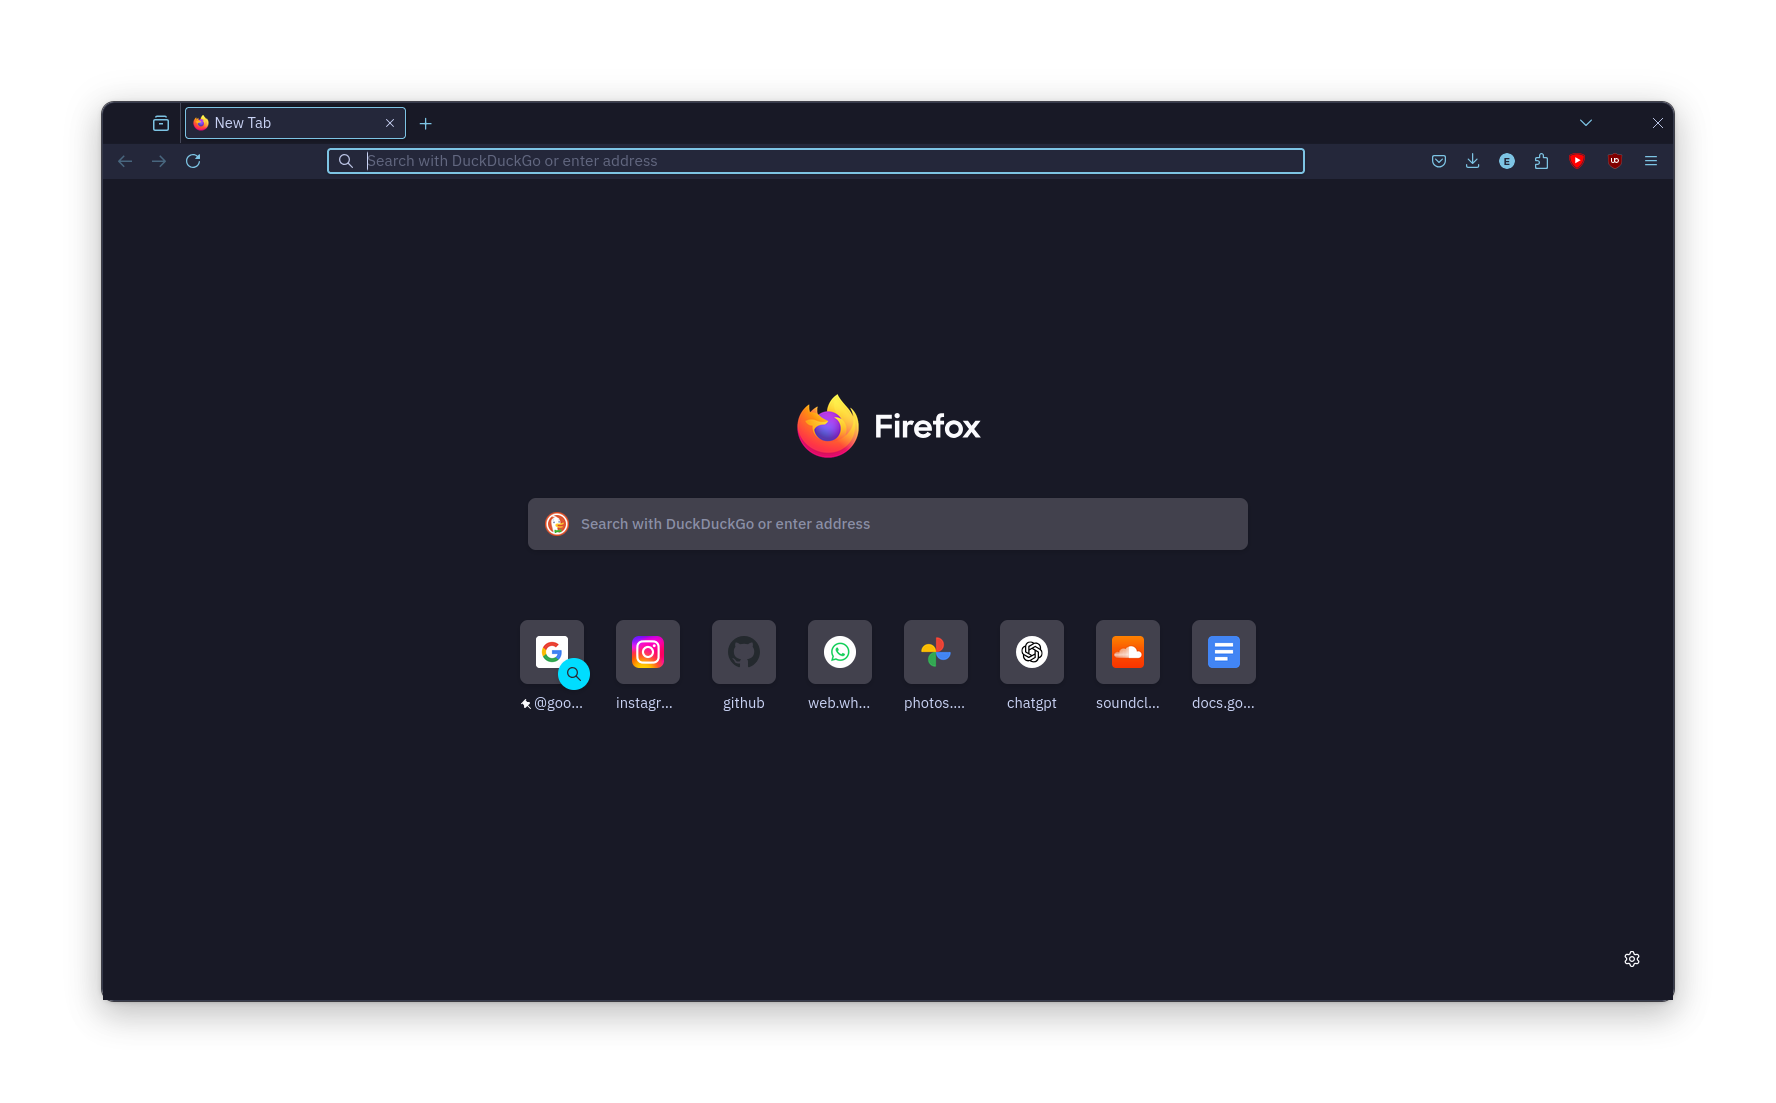
\includegraphics[width=0.8\textwidth]{firefox.png}
    \caption{A screenshot of the homescreen of the Firefox Browser.}
    \label{fig:firefox}
\end{figure}

They do several things:

\begin{itemize}
    \item Loads webpages at URLs.
    \item Keeps a history of all the website the user visited.
    \item They allow the user to navigate forward and backward.
    \item They make use of cookies.
    \item They support hyperlinks, which are links to other webpages/locations on the document.
    \item Data is stored inside of a cache.
\end{itemize}

and more.

\subsection{Loading Website Data}

In order to load HTML data from servers, it must find the IP address of the server first. However, website names are typed into the browser in their domain form, and not the IP address form. It must go through a \textbf{DNS} (Domain Name Server) first, which is (essentially) a large lookup table between domains and IP addresses. The typical procedure for your computer to load data from a server looks as follows:

\begin{figure}[H]
    \centering
    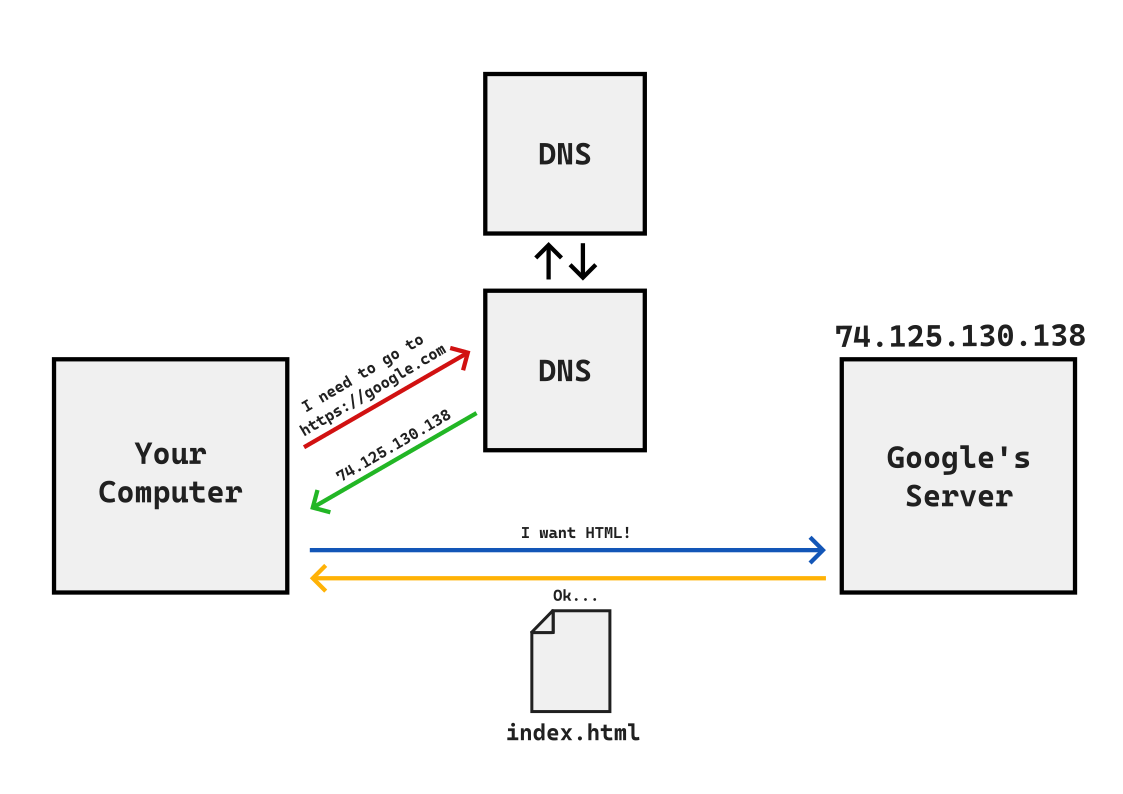
\includegraphics[width=0.8\textwidth]{dns.png}
    \caption{How a DNS works.}
    \label{fig:dns}
\end{figure}

\begin{enumerate}
    \item \textcolor{red}{Your computer requests the DNS for the IP address of the URL, in this case Google.com.}
    \item \textcolor{green}{The DNS may communicate with other nearby DNSes, and returns to the computer the IP address that your computer needs to load the resource.}
    \item \textcolor{blue}{Your computer then requests that webpage from the server, in this case Google.}
    \item \textcolor{yellow}{The server then responds with the corresponding data.}
\end{enumerate}

\subsection{Cookies}

These are like blobs used to store tempoary, small bits of information that relate to a website and its features.

In summary, cookies:

\begin{itemize}
    \item Allows websites to remember user data, including emails and payment information, so that they don't have to reinsert it into the website every time it's needed.
    \item Are used as memory for webpages, like a webpage's memory on the user's computer used all for itself.
    \item Can track internet habits and web histories, along with other personal information.
    \item Can be used in targeted advertising.
    \item Stores user preferences (like dark mode, etc.)
\end{itemize}

There are 2 main kinds of cookies, and they are as follows:

\paragraph{Session Cookies}

These are the most common type of cookie. These don't have an expiry date attached to it, and they are stored in RAM a not to the disk. Hence, they only exist when the browser is left open.

An example of session cookies use would be the shopping basket on a shopping site like Lazada. When you add items to the cart, it stores the contents of the cart in a cookie, so that when you relaod the page or visit other items, the cart is not emptied. They do not actually collect any information about the computer and do not identify the user.

\paragraph{Persistent Cookies}

Unlike session cookies, these persist by being stored on disk. These are usually used to store website settings, like making ChatGPT stay in dark mode. These cookies have an expiry date. When the expiry date of a persistent cookie is reached, or if the user deletes it, only then is it cleared.

These are used for:

\begin{itemize}
    \item Saving personal information, like credit cards
    \item Tracking your preferences on websites
    \item Storing login details
\end{itemize}

And others. Persistent cookies allows the web server to not store as much data as they usually would need to, as things like login details can be stored on the user's computer and can be loaded every time the site is visited.

Since these remain on disk, they can be used to \textbf{target users} by sending these cookies to other websites for advertising. They can also track your browser history and other personal data. Hackers can target persistent cookies on disk to breach your data, as well.

\paragraph{Loading Cookies}

\begin{enumerate}
    \item Every time a page is loaded by your web browser, it looks for any cookies.
    \item When it finds cookies, it loads both the persistent cookies stored on disk and session cookies which are stored in RAM (tempoary).
    \item When the website is closed, the persistent cookie is backed up on secondary storage.
    \item When the web browser itself is closed, the session cookies are deleted from memory.
\end{enumerate}

For more details, see page 185 of the textbook.

\subsection{How SSL works}
\label{5:sec:ssl}

\emph{NOTE: This came up in the May/June 2025 paper.} The method described is not the simplified version as shown in the textbook. This is because the textbook version is vague. If you require a simpler explanation, refer to figure 5.23 \textbf{in the textbook.}

\paragraph{The detailed way}

\begin{enumerate}
    \item The client sends a request to the browser, sharing which encryption algorithms are supported.
    \item The server responds with its SSL certificate, and the encryption method that it chose.
    \item The client validates the certificate, and checks if it had expired, and was issued by a trusted certificate authority.
    \item The client generates a session key for encryption, and encrypts it with the server's public key. It is sent to the server.
    \item The client and the server now have the same session key, which is used to both encrypt and decrypt data during the session. \emph{This session key is symmetric, as asymmetric encryption is expensive.}
\end{enumerate}

\end{document}
